Para $\mathbf{F}(x,y)=\langle-y,x\rangle$, construya una parametrización de la trayectoria mostrada y evalúe $\int_C\mathbf{F}\cdot d\vec r$.
\begingroup
\shorthandoff{>}
\begin{center}
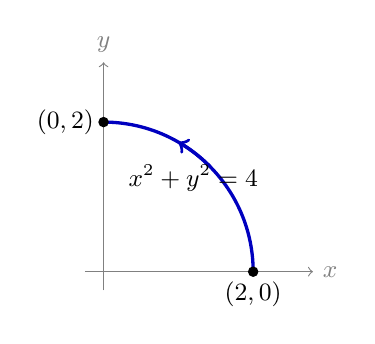
\begin{tikzpicture}[scale=.95,every node/.style={font=\small}]
    \draw[->,gray] (-.25,0)--(2.8,0) node[right] {$x$};
    \draw[->,gray] (0,-.25)--(0,2.8) node[above] {$y$};
    \draw[blue!75!black,very thick] (2,0) arc (0:90:2);
    \draw[blue!75!black,very thick,->] (45:2) arc (45:60:2);
    \fill (2,0) circle (2pt) node[below] {$(2,0)$};
    \fill (0,2) circle (2pt) node[left] {$(0,2)$};
    \node at (1.2,1.25) {$x^2+y^2=4$};
\end{tikzpicture}
\end{center}
\endgroup
